%%%
%%% FORMAL GAP IDENTIFICATION
%%%
\section{Gap between Synchronizing and Ordinary Transformations}

\todo{Exchange "ordinary" with "unidirectional"}
We have already introduced that there is both a formal and practical gap between synchronizing transformations, as we have defined as a component of transformation networks, and ordinary transformations, which are unidirectional and non-synchronizing, as used by most transformation languages.
In the following, we first give an example for faulty behavior if we simply used ordinary transformations in a transformation network.
Afterwards, we discuss options to sequence ordinary transformations and finally come up with a precise description of the formal gap and a practical approach to close it.

%%
%% MOTIVATING FAULT EXAMPLE WITH ORDINARY TRANSFORMATIONS
%%
\subsection{Behavior of Ordinary Transformations in Networks}
We have already sketched the example of creating a class in UML and Java after adding a component to a \gls{PCM} model in \autoref{chap:introduction:challenges:correctness:synchronization}.
In that scenario, it was possible that for a created \gls{PCM} component first a UML class is generated, which is then transformed into a Java class.
Additionally, the transformation between \gls{PCM} and Java creates another Java class, as it does not consider that there may be another transformation that already created that class.
Such scenarios can lead to the duplication of elements, or, in case of Java, an overwrite of an already created element, because the source file of the class will be placed at the same location in the file system.
Overwriting the previously created file may also overwrite and thus remove information that was already added to that class by the transformations across UML.

\begin{figure}
    \centering
    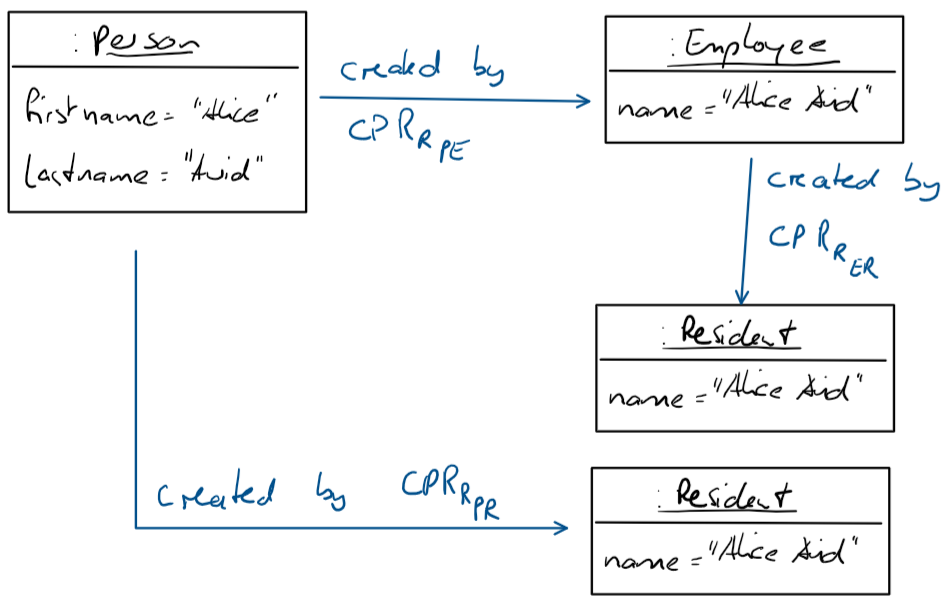
\includegraphics[width=0.8\textwidth]{figures/correctness/synchronization/duplicate_creation_example.png}    
    \caption{Duplicate creation of a resident by two sequences of consistency preservation rules}
    \label{fig:synchronization:duplicate_creation_example}
\end{figure}

An analogous example can be given for the running example of persons, employees and residents depicted in \autoref{fig:networks:three_persons_example}.
We consider the consistency relations $\consistencyrelation{R}{PE}, \consistencyrelation{R}{ER}$ and $\consistencyrelation{R}{PR}$.
As discussed in \autoref{chap:compatibility}, these relations are compatible, thus for any given person, employee or resident, there is a consistent set of models containing it.
Thus, the relations do not prevent transformations from finding consistent models whenever a person, employee or resident is added.
If we now consider ordinary transformations with unidirectional consistency preservation rules, they react to the changes in one model and update another accordingly.
In case of adding a person, this may look as depicted in \autoref{fig:synchronization:duplicate_creation_example}.
For each of the given consistency relations, we assume unidirectional consistency preservation rules that preserve consistency according to them.
They especially create an employee for each added person, and a resident for each created employee and person, respectively.
Since the transformations assume the models to be consistent before applying the changes, they always add a corresponding element when one of the elements is added.
This leads to the situation that both $\consistencypreservationrule{\consistencyrelation{CR}{ER},\rightarrow}$ as well as $\consistencypreservationrule{\consistencyrelation{CR}{PR},\rightarrow}$ create a resident upon creation of a person.
In consequence, there exist two residents with the same name, which does not fulfill the consistency relations.

It is our goal to find out how such a situation can be avoided by proper definition of consistency preservation rules in existing transformation languages.
A simple solution in this example would have been to look for the existence of elements to create first.
This can either be done by using a trace model, which most existing transformation language use to store corresponding elements, or by searching for an appropriate element in the other model.
Using a trace model, however, has some drawbacks and pitfalls, which we will investigate later.


% \begin{copiedFrom}{DocSym}

% % \section{Binary Transformation Interoperability}

% % Multi-model consistency preservation can be a achieved by combining binary transformations to graphs, %of transformations, 
% % with the transformations being executed transitively.
% % Since all binary transformations are developed independently of each other, it is necessary that they interoperate properly in a \emph{non-intrusive} way, thus without the necessity for the developer to understand and modify them, which we refer to as \emph{black-box combination}.

% Even under the assumption that, in contrast to our introductory motivation, all specifications are free of contradictions, it is easy to see that problems arise when combining binary transformations by transitively executing them.
% For example, consider the relations in \autoref{fig:prologue:binary_combination_example}.
% If a component is added to the \ac{ADL}, causing a \ac{UML} class creation due to \ref{fig:prologue:binary_combination_example:R1}, which in turn causes a Java class creation due to \ref{fig:prologue:binary_combination_example:R2}, the transformation for relation \ref{fig:prologue:binary_combination_example:R3} does not know that an appropriate class was already created, if the transformations are treated as black boxes.
% Consequently, the transformation will create the same class again, which may override the existing one, depending on the implementation and execution order.
% A simple solution for this example would be to have all transformations use a common trace model and check for existing elements before creating them in a transformation.
% Nevertheless, independently developed transformations will usually not assume that %this only applies if the transformation considers possibly preexisting transformation results, which it will not do in general if it does not assume other transformations to create corresponding elements.
% other transformations may already have created corresponding elements.
% Additionally, the trace model must allow the transformation engine to retrieve transitive traces.
% However, it is unclear if transitive resolution of traces can always be performed, as it can depend on whether the transitive trace belongs the considered consistency relation or another.
% %If, in another scenario, the transformation in the example was actually supposed to create an additional class, it would have to ignore the existing trace.

% As can be seen in the example, especially the correct handling of trace information in interdependent transformations has to be researched.
% This applies not only to element creations, but also other change types, such as attribute or reference changes, especially if they are multi-valued.
% In our thesis, we will therefore apply transitively executed binary transformations in different case studies to identify these and potential further problems.
% We then want to come up with a catalog of such problems %preventing the black-box combination of transformations 
% together with solution patterns for them.
% For example, to avoid duplicate element creations, a simple pattern could be to always check for already existing traces for that consistency relation in the transformations.
% In consequence, the integration of those patterns into a transformation language or the application of them as a transformation developer is supposed to achieve black-box combinability of the transformations.

% \end{copiedFrom} % DocSym


\subsection{Consistency Preservation for Fine-grained Relations}

\mnote{Consistency preservation defined for model-level consistency relations}
In our definition of consistency preservation rules in \autoref{def:consistencypreservationrule}, we used the coarse-grained notion of \modellevelconsistencyrelations, which describes consistency between two models in terms of a single relations.
In consequence, such a \modellevelconsistencypreservationrule ensures consistency to a single consistency relation.

\mnote{Fine-grained consistency relations allow to define relation between unidirectional preservation rules}
In \autoref{chap:compatibility:formal_notion}, we discussed that consistency relations can be considered in a fine-grained way that is able to reflect different notion of consistency in both directions of a relation.
We thus refined the notion of consistency relations in \autoref{def:consistencyrelation} to be defined at the level of model elements rather than complete models.
%This fine-grained notion of consistency does also fit well to how specifications in transformation languages consider consistency, as they define rules that relate only some classes by relations or routines to preserve their consistency.
We thus base further consideration on consistency preservation rules on such fine-grained consistency relations.
Nevertheless, we did also discuss in that chapter that all fine-grained relations can also be translated into \modellevelconsistencyrelations, thus all insights we already had for those model-level relations still apply to the considerations regarding fine-grained ones.

\mnote{Transformation languages use fine-grained relations and preservation rules}
This fine-grained notion of consistency does also fit well to how specifications in transformation languages consider consistency.
They allow to define rules that relate only some classes by relations, conforming to fine-grained consistency relations, from which then fine-grained consistency preservation rules are derived, or they directly allow to define routines to preserve consistency between specific classes.
These rules are often called \emph{transformation rules} and composed to a transformation that consists of multiple such rules, each encoding a consistency relations and a preservation rule for it.
%We will, however, stick to the coarse-grained notion of consistency preservation rules, because, first, it is difficult to describe how such fine-grained consistency preservation rules can be composed, and second, the coarse-grained notion is sufficient for our considerations anyway.

\mnote{Stick to coarse-grained notion of preservation rules}
It may happen easily that the execution of one transformation rule leads to the violation of the consistency relation of another one, which introduced dependencies between the individual transformation rules.
Thus, a combination of such transformation rules to a transformation has to ensure correctness, i.e., that the consecutive execution of the rules leads to a consistent state of the models.
Languages such as \gls{QVTR} and \gls{QVTO} therefore precisely specify in which order single transformation rules can and need to be executed. \todo{Add reference}
It is also a dedicated topic of research to ensure that the rules of a single transformation conform to each other \todo{Add references}, thus we assume that a transformation has that property.
To avoid the necessity of specifying this conformance property for transformation rules, we stick to the existing notion of coarse-grained consistency preservation rules, as it is sufficient for our considerations.

\mnote{New transformation notion based on fine-grained consistency relations}
In consequence, from now we will consider a synchronizing transformation as a set of fine-grained consistency relations according to \autoref{def:consistencyrelation} and a consistency preservation rule that preserves consistency according to the set of relations $\consistencyrelationset{CR}$ rather than a single \modellevelconsistencyrelation $\consistencyrelation{CR}{}$.
The consistency preservation rule $\consistencypreservationrule{\consistencyrelationset{CR}}$ and also the complete transformation are thus still considered correct if applying it to a consistent pair of models and changes to them, applying the resulting changes to the models again delivers a pair of models that is consistent to all consistency relations, i.e.:
\begin{align*}
    &
    \forall \model{m}{1} \in \metamodelinstanceset{M}{1}, \model{m}{2} \in \metamodelinstanceset{M}{2}, \change{\metamodel{M}{1}} \in \changeuniverse{\metamodel{M}{1}}, \change{\metamodel{M}{2}} \in \changeuniverse{\metamodel{M}{2}} : \tupled{\model{m}{1},\model{m}{2}} \consistenttomath \consistencyrelationset{CR} \\
    & \formulaskip
    \land \exists \change{\metamodel{M}{1}}' \in \changeuniverse{\metamodel{M}{1}}, \change{\metamodel{M}{2}}' \in \changeuniverse{\metamodel{M}{2}} : \tupled{\change{\metamodel{M}{1}}', \change{\metamodel{M}{2}}'} = \consistencypreservationrule{\consistencyrelationset{CR}}(\model{m}{1}, \model{m}{2}, \change{\metamodel{M}{1}}, \change{\metamodel{M}{2}}) \\
    & \formulaskip\formulaskip
    \Rightarrow \tupled{\change{\metamodel{M}{1}}'(\model{m}{1}),\change{\metamodel{M}{2}}'(\model{m}{2})} \consistenttomath \consistencyrelationset{CR}
\end{align*}
Note that being consistent to all fine-grained consistency relations is equivalent to being consistent to the single \modellevelconsistencyrelation induced by the fine-grained relations.

% In our definition of consistency preservation rules in \autoref{def:consistencypreservationrule}, we used the coarse-grained notion of \modellevelconsistencyrelations and, accordingly, defined \modellevelconsistencypreservationrules that consider models as whole.
% We refined the notion of consistency relations in \autoref{def:consistencyrelation} to be defined at the level of model elements rather than complete models.
% This fine-grained notion of consistency fits well to how specifications in transformation languages consider consistency, as they define rules that relate only some classes by relations or routines to preserve their consistency.
% In the following, we thus also stick to this fine-grained notion of consistency.
% We will, however, stick to the coarse-grained notion of consistency preservation rules given in \autoref{def:consistencypreservationrule}

% \subsection{Feingranulare CPR}
% Jede CPR stellt Konsistenz bzgl. einer unidirektionalen CR wieder her.
% Ein CPR darf keine Änderung machen, die eine andere CR verletzt.
% Schwierig, da CPR voneinander abhängen können (was wiederum dagegen spricht, dass eine CPR nicht eine andere CR verletzen darf), wie also Reihenfolge festlegen?
% Ist keine Option, insbesondere Annahme, dass sich CPR nicht gegenseitig beeinflussen nicht nachvollziehbar (obwohl in der Praxis dasselbe Probleme existiert, da CPR sowieso in feingranulare Regeln zerlegt werden, die natürlich widersprüchlich sein könnten).



\subsection{Unidirectional Consistency Preservation Rules}

\mnote{Formal definition of unidirectional consistency preservation rules}
Before discussing options how unidirectional consistency preservation rules can be used to emulate the behavior of synchronizing consistency preservation rules, we first need to define them to formally compare the two of them.
In contrast to a synchronizing consistency preservation rule as defined in \autoref{def:consisistencypreservationrule}, a unidirectional consistency preservation rule does only receive changes made to one of the two models and returns changes to the other models instead of receiving and returning changes to both.

\begin{definition}[Unidirectional Consistency Preservation Rule]
    \label{def:unidirectionalconsistencypreservationrule}
    Let $\metamodel{M}{1}, \metamodel{M}{2}$ be two metamodels and $\consistencyrelationset{CR}$ a set of consistency relations between elements of those metamodels.
    A \emph{unidirectional consistency preservation rule} $\consistencypreservationrule{\consistencyrelationset{CR}}$ for the relation set $\consistencyrelationset{CR}$ is a function:
    \begin{align*}
        \consistencypreservationrule{\consistencyrelationset{CR}} : (\metamodelinstanceset{M}{1}, \metamodelinstanceset{M}{2}, \changeuniverse{\metamodel{M}{1}}) \rightarrow \changeuniverse{\metamodel{M}{2}}
    \end{align*}
\end{definition}

\mnote{Preservation rules as defined in or derived in transformation languages}
This is how the consistency preservation rules defined in or derived from existing transformation languages operate.
They take two models and changes to one of them and generate changes for the other.
Most of them even directly apply the changes instead of returning a dedicated change artifact.

\mnote{Correctness of unidirectional rules analogous to common notions}
In addition, they usually assume the input models to be consistent and then ensure that applying the input and the output changes to the models, the resulting models are consistent again.
This conforms to the common notion of \emph{correctness} for consistency preservation rules, like for the state-based (rather than our delta-based) notion of consistency preservation rules defined in \autoref{stevens2010sosym}.
This is even compliant to the correctness notion that we defined for synchronizing consistency preservation rules in \autoref{def:consistencypreservationrulecorrectness}.
Thus, we define correctness of such a unidirectional consistency preservation rule as follows.

\begin{definition}[Unidirectional Consistency Preservation Rule Correctness]
    \label{def:unidirectionalconsistencypreservationrulecorrectness}
    Let $\consistencypreservationrule{\consistencyrelationset{CR}}$ be a \emph{unidirectional consistency preservation rule}.
    We call $\consistencypreservationrule{\consistencyrelationset{CR}}$ \emph{correct} if the resulting models when applying the generated changes are consistent to $\consistencyrelationset{CR}$ again:
    \begin{align*}
        &
        \forall 
        \model{m}{1} \in \metamodelinstanceset{M}{1}, 
        \model{m}{2} \in \metamodelinstanceset{M}{2},
        \change{\metamodel{M}{1}} \in \changeuniverse{\metamodel{M}{1}} : \\
        & \formulaskip
        \tupled{\model{m}{1}, \model{m}{2}} \consistenttomath \consistencyrelationset{CR} \\
        & \formulaskip
        \land \exists 
        \change{\metamodel{M}{2}} \in \changeuniverse{\metamodel{M}{2}} :
        \change{\metamodel{M}{2}} = \consistencypreservationrule{\consistencyrelation{CR}{}}(\model{m}{1}, \model{m}{2}, \change{\metamodel{M}{1}}) \\
        & \formulaskip\formulaskip
        \Rightarrow
        \tupled{\change{\metamodel{M}{1}}(\model{m}{1}), \change{\metamodel{M}{2}}(\model{m}{2})} \consistenttomath \consistencyrelationset{CR}
    \end{align*}
\end{definition}


\subsection{Bidirectional Transformations}

In practice unidirectional CPR are defined as pairs for both directions. This is usually denoted as bidirectional transformations.
They properly work for both directions individually.
\todo{Define Bidirectional Transformation, being composed of two unidirectional ones. Define correctness for the case that only one model was modified.}


\subsection{Alignment of Unidirectional Relations and Preservation}
A unidirectional consistency relations require preservation rules in both directions (add/delete)
\begin{itemize}
    \item A single unidirectional consistency relation may impose preservation rules in both directions: For each employee, a resident is required, but not every resident needs to be an employee. When then have only one unidirectional consistency relation describing that circumstance. We need, however, consistency preservation rules in both directions, because if, for example, a resident is removed, the employee needs to be removed as well, whereas a resident has to be added whenever an employee is added.
    \item With ordinary unidirectional rules, we then have that after a change to model 1, the unidirectional rule has to change model 2 so that they are consistent to both unidirectional relations (and vice versa)
\end{itemize}
Konsequenz: Wir können nicht für die unidirektionalen Konsistenzrelationen jeweils die CPR in die Richtung angeben, sondern jede unidirektionale CPR muss immer die Konsistenzrelationen in beide Richtungen berücksichtigen.

Define mapping between change types and directionality of involved consistency relation (delete in opposite direction than add or modification). Make example at witness structures.


\paragraph{Synchronizing Transformation cannot be Unidirectional}
Es ist einfach zu sehen, dass synchronisierende Transformationen nicht so einfach unidirektional definiert werden können.
Wird m1 beliebig geändert und in m2 ein Element gelöscht, welches für Konsistenz zu m1 notwendig war, dann kann die unidirektionale CPR m2 nicht wieder so anpassen, dass es konsistent zu m1 ist, außer indem es das gelöschte Element wieder hinzufügt. Hier wäre es richtig das Element in m1 durch die gegenläufige CPR zu löschen. 
Das bedeutet aber das Korrektheit hier nicht definiert werden kann als die Eigenschaft Konsistenz bzgl. aller CR durch eine unidirektionale CPR herzustellen.

Das gilt allerdings nur, wenn man den Korrektheitsbegriff beibehält. Wir werden sehen, dass es andere Möglichkeiten gibt diesen Begriff einer unidirektionalen synchronisierenden Transformation zu definieren.


\subsection{Partial Definition of Consistency Preservation Rules}
1. Schon eine synchronisierende Transformation muss nicht für jede Eingabe definiert sein. Es könnte natürlich sein, dass sich gleichzeitige Änderungen nicht sinnvoll in Einklang bringen lassen. Theoretisch ist es aber möglich eine total definierte Funktion anzugeben, da immer ein beliebigen (im dümmsten Fall immer dasselbe / leere Modell) zurückgeliefert werden kann.

\todo{Conclude that an open issue is how to combine to unidirectional CPRs to emulate a synchronizing transformation, i.e. react to changes in both models.}





\section{Combining Unidirectional Consistency Preservation Rules}

%%
%% OPTIONS TO COMBINE TRANSFORMATIONS
%%
\subsection{Options for Consistency Preservation Rule Combination}

\mnote{Existing synchronization supports arbitrary conflicting concurrent changes}
Some existing work already proposed strategies to synchronize concurrent changes between two models.
For example, some work proposes techniques for processing concurrent changes with \glspl{TGG}~\cite{hermann2012concurrentSynchronization-FASE,orejas2020IncrementalConcurrentSynchronization-FASE}, whereas others define specific algorithms for a general notion of synchronizing transformations according to our given definition~\cite{xiong2013SynchronizingConcurrentUpdates-SoSym,xiong2009parallelUpdates-ICMT}.
All these approaches, however, deal with the more general case that any changes may have been made to the models.
That especially includes conflicting updates by one or more user, which need to be resolved.
Such a resolution may lead to the necessity of reverting one of the changes.

\mnote{Transformation networks only produce specific concurrency situations}
We are, however, in the special situation that transformations do not perform arbitrary changes and that changes of other transformations may need to be revised, but not reverted.
For example, it may be necessary to update an attribute value again, because the interval of consistent values of the currently executed transformation is smaller than the one of a transformation executed before.
It will, however, not be necessary to completely revert the modification of the attribute value, because the modification was necessary for another transformation to restore consistency, thus the causal change for which consistency was restored, needs to be reverted as well.
Finally, this would result in reverting a user change, which should never happen.

\mnote{We assume compatibility of transformations}
In fact, we assume transformations to be compatible according to \autoref{def:compatibility}, which excludes contradictions in their consistency relations that may prevent transformations from being able to find a consistent result for specific changes.
This assumptions reduces the potential conflicts that may occur when changes of different transformations need to be synchronized.

\mnote{Difference between synchronizing and unidirectional consistency preservation rules}
A synchronizing consistency preservation rule according to \autoref{def:consistencypreservationrule} receives two models and two changes, one for each of the models, and returns two changes, i.e.:
\begin{align*}
    \consistencypreservationrule{\consistencyrelation{CR}{}} : (\metamodelinstanceset{M}{1}, \metamodelinstanceset{M}{2}, \changeuniverse{\metamodel{M}{1}}, \changeuniverse{\metamodel{M}{2}}) \rightarrow (\changeuniverse{\metamodel{M}{1}}, \changeuniverse{\metamodel{M}{2}})
\end{align*}
%\todo{Maybe add this to correctness formalization: Give example why we need that: both models can be modified due to network, both may need to be modified because if in both models something is added that needs to be reflected in the other, both have to be changed to restore consistency, without reverting one of the changes.}
%We used this rather general notion of a consistency preservation rule between two metamodels to support that both models may have been modified, which is inevitable in a transformation network.
%Additionally, both models may need to be modified to properly consistency.
It would, however, be a cumbersome task to define the behavior of the transformation, or more precisely its consistency preservation rule, for all potential pairs of changes in both models.
Furthermore, existing transformation languages usually specify unidirectional consistency preservation rules, thus they only support the propagation of changes made in one model to the other, but not to process changes made to both models at once. Thus, each bidirectional transformation defined in a transformation language actually consists of two consistency preservation rules:
\begin{align*}
    \consistencypreservationrule{\consistencyrelation{CR}{},\rightarrow} : (\metamodelinstanceset{M}{1}, \metamodelinstanceset{M}{2}, \changeuniverse{\metamodel{M}{1}}) \rightarrow \changeuniverse{\metamodel{M}{2}}\\
    \consistencypreservationrule{\consistencyrelation{CR}{},\leftarrow} : (\metamodelinstanceset{M}{1}, \metamodelinstanceset{M}{2}, \changeuniverse{\metamodel{M}{2}}) \rightarrow \changeuniverse{\metamodel{M}{1}}
\end{align*}

\mnote{First option: Independent execution and merge}
In consequence, we usually have two unidirectional consistency preservation rules $\consistencypreservationrule{\consistencyrelation{CR}{},\rightarrow}$ and $\consistencypreservationrule{\consistencyrelation{CR}{},\leftarrow}$ that define how changes are propagated from one model to the other and vice versa, but this is not equivalent to a synchronizing transformation.
Imagine models $\model{m}{1}$ and $\model{m}{2}$ and changes to them $\change{\metamodel{M}{1}}$ and $\change{\metamodel{M}{2}}$.
If we now applied the two unidirectional consistency preservation rules independently, we would have $\change{\metamodel{M}{2}}' = \consistencypreservationrule{\consistencyrelation{CR}{},\rightarrow}(\model{m}{1},\model{m}{2}, \change{\metamodel{M}{1}})$ and $\change{\metamodel{M}{1}}' = \consistencypreservationrule{\consistencyrelation{CR}{},\leftarrow}(\model{m}{1},\model{m}{2}, \change{\metamodel{M}{2}})$.
It is, however, not guaranteed that $\tupled{\change{\metamodel{M}{1}}' \concatfunction \change{\metamodel{M}{1}}(\model{m}{1}), \change{\metamodel{M}{2}}' \concatfunction \change{\metamodel{M}{2}}(\model{m}{2})}$ is consistent, thus simply merging the individually produced changes does not necessarily lead to a consistent result.

\mnote{Second option: Sequential execution}
Another option would be to sequence the execution, thus first generating $\change{\metamodel{M}{2}}' = \consistencypreservationrule{\consistencyrelation{CR}{},\rightarrow}(\model{m}{1},\model{m}{2}, \change{\metamodel{M}{1}}$ as before.
Afterwards, we apply the second consistency preservation rule to modified $\model{m}{2}$, thus $\change{\metamodel{M}{1}}' = \consistencypreservationrule{\consistencyrelation{CR}{},\leftarrow}(\change{\metamodel{M}{1}}(\model{m}{1}),\change{\metamodel{M}{2}}'(\model{m}{2}), \change{\metamodel{M}{2}})$.
As a result, we receive $\tupled{\change{\metamodel{M}{1}'} \concatfunction \change{\metamodel{M}{1}}(\model{m}{1}, \change{\metamodel{M}{2}} \concatfunction \change{\metamodel{M}{2}}'(\model{m}{2})}$, which is consistent to $\consistencyrelation{CR}{}$.
This means that $\change{\metamodel{M}{2}}$ is not applied to $\model{m}{2}$ anymore, to which the changes were made originally, but needs to be applied to $\change{\metamodel{M}{2}}'(\model{m}{2})$.
It is, however, not clear whether the change can still be applied to that state, i.e., whether $\change{\metamodel{M}{2}}$ is defined for $\change{\metamodel{M}{2}}'(\model{m}{2})$.
An example may be that $\change{\metamodel{M}{2}}'$ removes an element from $\model{m}{2}$, which $\change{\metamodel{M}{2}}$ changes.
\todo{Revise change definition to be partial}

\mnote{Goal is to preserve all original changes}
We, however, want to ensure that both original changes are applied to the models and consistency preservation rules can react to them.
Thus, we aim to find an approach that allows the unidirectional consistency preservation rules to also deal with the situation that the both models have been modified to emulate a synchronizing rule.



\subsection{Sequencing of Consistency Preservation Rules}

Optimalfall: d2' und d2 erzeugen Änderungen für Elemente, die disjunkte Mengen von Condition Elements betreffen. Dann können sie beliebig sequentialisiert werden und erzeugen konsistente Ergebnisse.

Problemfälle:
d2' erzeugt Änderungen, die sich nicht auf d2 anwenden lassen
d2' erzeugt Änderungen, die sich auf Condition Elemente beziehen, die von d2 geändert werden
d2' und d2 erzeugen Änderungen, die zusammen neue Condition Elements induzieren

\begin{itemize}
    \item In the best case we would apply changes to model 1, then execute the first preservation rule to change model 2 (so they are consistent then again) and then apply the changes to model 2 and execute the second preservation rule, such that they are then consistent again.
    \item What comes in mind directly: For sure, this could result in the situation that changes are reverted, because the change to 1 propagated by 1 -> 2 changes a value which is changed by back by change to 2 and then reverted back by 2 -> 1. But even a synchronizing transformation would have to select either of the values in that case and revert one the changes, so there is already an underlying problem of the relations that may not be compatible
    \item It is however unclear whether the changes to model 2 can still be applied after applying the changes of the transformation 
    \item We therefore make a case distinction over all possible combinations of changes to be executed one after another.
    \item Especially, we want to find out where there are conflicts if changes to model 2 are applied before 1 -> 2 changes. This allows us to encode 1 -> 2 in a way that it is able to deal with it instead of having the problem of not being able to apply changes to model 2
\end{itemize}

Kann d2 auf d2' angewendet werden? Was sind mögliche Probleme?
%Wir können Sequentialisieren, aber dann sind Änderungen potentiell nicht mehr propagierbar (und wenn die CPR es doch tun, weil sie für die Eingabe undefiniert sind und irgendwas tun, kommt Quatsch raus).

1. Nicht Anwendbarkeit: Element, auf das Änderung angewendet werden soll, existiert nicht mehr. D.h. das Element wurde durch die CPR entfernt, was nötig war, um die entsprechende Konsistenzrelation zu erfüllen. Die Änderung die über einen anderen Pfad kam, kann nicht mehr angewendet werden. Das Condition Element ist nicht mehr vorhanden, also muss diese Löschung zurückpropagiert werden, damit auch entsprechend der anderen Konsistenzrelationen die korrespondierenden Condition Elements entfernt werden -> Änderung wird ignoriert und die Löschung wird propagiert
2. Nicht Propagierbarkeit (gilt generell für die Propagierbarkeit von Änderungen, nicht nur in diesem Szenario, auch bei Nutzeränderungen): Wenn alle Änderungen angewendet sind, kann der Zielzustand so sein, dass d1(m1) nicht so angepasst werden, dass Konsistenz wiederherstellt wird. Dies ist insbesondere dann der Fall, wenn für d2(d2'(m2)) kein Modell in IM1 existiert, sodass es eine valide Witness-Struktur gibt. Das ist dann der Fall, wenn nicht für jedes Condition Element ein eindeutiges korrespondierendes gefunden werden kann, also entweder aufgrund der Elemente in d2(d2'(m2)) in einem m1 Elemente vorkommen müssen, die durch eine Konsistenzregel ein weiteres Condition Element in d2(d2'(m2)) benötigen würden, oder es kein m1 gibt, sodass eine eindeutige Zuordnung möglich ist, also in d2(d2'(m2)) quasi doppelte Elemente vorkommen

Ersteres wäre bspw. der Fall, wenn ein zweiter Resident eingefügt wird, dafür entsprechend ein zweiter Employee erzeugt werden muss, aber bei zwei Employees (warum auch immer) immer ein dritter Resident erzeugt werden muss, durch eine weitere Konsistenzrelation. Dies wäre jedoch auch ein Problem, wenn der Nutzer eine solche Änderung macht, da dann die CPR gar nicht in der Lage ist unidirektional Konsistenz herzustellen. Daher können wir mit solch einer Art von  Konsistenzrelationen sowieso per se nicht umgehen. Wie bereits gesagt, kann man das in der Praxis dennoch erlauben und verliert dann gewisse Garantien bzgl. Konsistenz oder Terminierung. Der Entwickler muss das halt einfach richtig umsetzen.
Dieses Problem ließe sich noch durch mehrfache Ausführung der Transformationen lösen, da es immer noch Modelle gibt, die diese Änderung reflektieren und konsistent sind, muss eben nur die Transformationen dafür lange genung ausführen.

Zweiteres wäre beispielsweise ein doppelter Resident, für den kein konsistentes Employee-Modell erzeugt werden kann.
Das Vorkommen doppelter Elemente lässt sich auch nicht durch mehrfache Ausführung der CPR auflösen (außer man löscht eines der Elemente wieder).
Hier ist das zugrunde liegende Problem, dass mehrfach ein Element erzeugt wurde, was eigentlich das gleiche sein soll.
Eine synchronisierende Transformation könnte an dieser Stelle berücksichtigen, dass d2 bereits entsprechende Elemente einfügt, sodass in d2' nicht zusätzliche Erzeugungen generiert werden müssen, um eine valide Witness-Struktur zu induzieren.
Die unidirektionale CPR sieht diese Änderung jedoch nicht und somit passiert die Hinzufügung doppelt.
Um das zu Vermeiden müsste die CPR berücksichtigen, dass d2 bereits entsprechende Änderungen macht.

Go on here \dots


Wenn wir die undirektionalen CPR sequentialisieren (also erst d2' erzeugen, dann d2 darauf anwenden), kann es sein, dass d2'(m2) Änderungen an Condition Elements in m2 vornimmt oder neue hinzufügt, um Konsistenz wiederherzustellen, die ebenfalls von d2 eingefügt werden, sodass es nicht mehr möglich ist, durch die rückwärtige CPR Änderungen vorzunehmen, die eine valide Witness-Struktur induzieren.
Z.B. könnte d2'(m2) einen Resident hinzufügen, der bereits durch d2 eingefügt wurde (weil er über einen anderne Pfad erstellt wurde, siehe \autoref{fig:synchronization:duplicate_creation_example}). Wird nun d2 auf d2'(m2) angewendet, würde ggf. in einem Container, in dem die Residents gespeichert werden, zwei Residents mit gleichem Namen eingefügt. Für diese kann aber keine Änderung in m1 (sei es das Employee-Modell) erzeugt werden, durch die eine valide Witness-Struktur entsteht. Das Einfügen eines zweiten Employee mit dem gleichen Namen führt dazu, dass jeder Employee und jeder Resident zu zwei Residents bzw. Employees korrespondiert, was keine eindeutige Witness-Struktur induziert.
Um dies zu vermeiden, müssen die CPR sicherstellen, dass in den Änderungen am anderen Modell nicht bereits entsprechende Condition Elements erzeugt wurden.
Alle anderen Änderungen sind unproblematisch, da Änderungen die d2 an bestehenden Condition Elements, die nicht zu neuen Condition Elements führen, durchführt mittels 2->1 propagiert werden können, indem die Condition Elements in m1 angepasst werden.

Insgesamt ist die Situation die gleiche, als würde ein Nutzer eine entsprechende Änderung machen. Auch er kann natürlich einen zweiten Resident mit demselben Namen einführen. Hier würde die CPR selbstverständlich fehlschlagen. Während das für Nutzeränderungen erwüscht ist, da die doppelte Erzeugung desselben Elementes hier schon vom Nutzer durchgeführt wurde und für einen entsprechende Nutzeränderung kein konsistentes Modell generiert werden kann, ist dies innerhalb des Transformationsnetwerkes unerwünscht, da die CPR natürlich eine konsistente Modellmenge finden können und die doppelte Erzeugung lediglich daher kommt, dass die Transformationen nicht, wie verlangt, synchronisieren sind. In letztem Fall wäre sichergestellt, dass nach entsprechenden Änderungen an beiden Modellen (also Erzegung von Employee in einem, Erzeugung des passenden Resident im anderen) keine Änderungen gemacht werden, da bereits eine passende Witness-Struktur vorhanden ist.
Die unidirektionalen CPR schaffen das jedoch nicht, da Ihnen die entsprechende Information fehlt.

\paragraph{Concatenation of Changes}
WAS PASSIERT EIGENTLICH BEI CHANGE CONCATENATION?
Bis jetzt haben wir Änderungen immer nur auf den Zustand eines Modells angewandt, für den sie auch generiert waren. Ein Change kann jedoch von seiner Definition her auch auf andere Zustände angewandt werden. Die Frage ist, wie er sich dabei verhält. Die Definition macht dazu erstmal keine Aussage, d.h. er könnte im Prinzip beliebigen Quatsch machen. Natürlicherweise würde man aber erwarten, dass er dieselben Änderungen an Modellen durchführt (Einfügen/Löschen von Objekten, Ändern von Attributen/Referenzen usw.), soweit dies möglich ist. Zumindest wenn die jeweiligen Elemente vorhanden sind, auf die sich die Änderungen beziehen, sollte die Änderung das gleiche ausführen.
Da wir das nicht präzise formulieren können, kommen wir nicht umhin, dass d2' auf Basis von d2(m2) erzeugt wird. Also spricht auch das gegen Sequentialisierung.


\subsection{Non-termination of Bidirectional Transformations}

Wie bei Orchestrierung gesehen, kann es im Allgemeinen notwendig sein CPRs mehrfach auszuführen, da die aufeinander reagieren müssen, um eine konsistente Modellmenge "auszuhandeln".
Dasselbe kann bei zwei unidirektionalen Transformationen passieren. Während eine synchronisierende Transformation beliebige Änderungen an beiden Modellen machen kann, kann es sein, dass unidirektionale Transformationen mehrfach aufeinander reagieren müssen, um das gleiche zu erreichen.

\begin{figure}
    \centering
    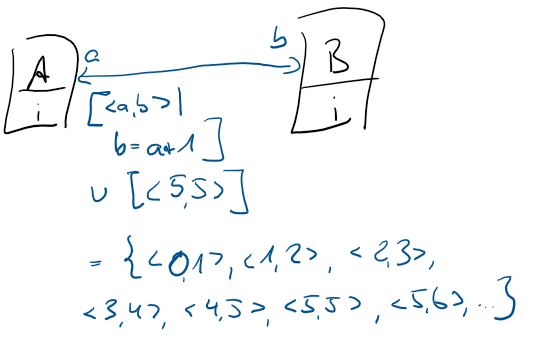
\includegraphics[width=0.8\textwidth]{figures/correctness/synchronization/multiple_unidirectional_execution.png}
    \caption[Multiple execution of unidirectional consistency preservation rules]{A consistency relation requiring multiple executions of unidirectional consistency preservation rules to find a consistent result}
    \label{fig:synchronization:multiple_unidirectional_execution}
\end{figure}

Siehe \autoref{fig:synchornization:multiple_unidirectional_execution}: Es gibt zwei Relationen (und deren transponierte). Die eine Relation ist erfüllt, wenn für jedes A mit einer Zahl ein B mit der Zahl um eins höher vorkommt, außer A ist 5 (oder eine bel. andere Zahl), dann darf B auch 5 sein (und umgekehrt). Die andere Relation ist erfüllt, wenn für jedes A ein B mit der gleichen Zahl existiert (und umgekehrt).
Wird nun A(i=0) in das Modell eingefügt, wird zur Erfüllung der Relationen B(i=1) und B(i=0) von der CPRr eingefügt.
Daraufhin fügt die CPRl A(i=1) ein, da sonst $CR_2$ nicht erfüllt ist.
Nun fügt CPRr wiederum B(i=2) ein, damit $CR_1$ erfüllt ist usw.
Dies geht bis CPRl A(i=5) einfügt, denn nun ist auch $CR_1$ erfüllt.
Es braucht mehrere Durchläufe um dieses Ergebnis zu erhalten.

Das folgende ist alles intuitiv gesprochen, funktioniert so nicht.
ERKENNTNIS: Wir können von einer unidirektionalen CPR i.A. gar nicht verlangen, dass sie Konsistenz bzgl. aller Relationen herstellt.
Ziel ist nur, dass sie die Konsistenzrelationen in Vorwärtsrichtung wiederherstellt, in Rückwärtsrichtung nicht vollständig.
Bspw. für ein Insert fügt sie Elemente hinzu, bei Änderung passt sie Elemente an. Bei einer Löschung ist die rückwärtige Konsistenzrelation nicht erfüllt, hier muss aber die CPR vorwärts löschen, d.h. wir verlangen, dass Elemente die vorher schon im Zielmodell waren und immer noch sind, auch konsistent sind bzgl. aller Relationen bzgl. der sie vorher konsistent waren.
Auch für eine Änderung gilt das in die Richtung: Wenn ich an m1 was ändere wodurch eine Witness-Struktur in Rückrichtung verletzt wird, muss die vorwärts CPR das wiederherstellen.

Das bedeutet, die rückwärts CPR muss dann nur noch auf Hinzufügungen oder Änderungen reagieren, die durch die vorwärts CPR gemacht wurden (auch Löschungen?).
ERKENNTNIS: Wir können noch nicht einmal Terminierung für zwei unidirektionale Transformationen garantieren. Letztendlich haben wir dort wieder das gleiche Problem wie in Netzwerken, wie wir im Orchestrierungs-Kapitel sehen werden. Das Beispiel zeigt, dass es auch keine obere Schranke für die Anzahl aus Ausführungen gibt (je nach Wahl von X sind hier beliebig viele möglich). Wir könnten Sie nur eine gewissen Zeit ausführen lassen und ansonsten konservativ abbrechen.

ALSO: Entweder lassen wir das zu, dann können wir keine Terminierung erwarten, oder wir fordern halt, dass eine CPR immer in einem Schritt Konsistenz herstellen muss (für alle Relationen) und wenn sie das nicht schafft, wirft sie eben einen Fehler. Dadurch sind manche Fälle ausgeschlossen, aber das macht man üblicherweise ja immer so.

WAS TUN WIR?
Wir verlangen das was alle Formalismen bisher verlangen: Eine unidirektionale CPR kann vollständig Konsistenz herstellen. Auch wenn es theoretische Szenarien gibt, in denen das nicht möglich ist, gehen bisher diverse Arbeiten davon aus und in unserer Evaluation (siehe \autoref{chap:correctness_evaluation}) werden wir sehen, dass es auch in unseren Fallstudien der Fall ist.
AUßERDEM: In der Praxis können wir natürlich solche Szenarien erlauben, auch wenn dann gewisse Eigenschaften auf Basis des Formalismus nicht mehr garantiert sind.
Wenn der Entwickler die Transformationen so baut, dass deren mehrfache Ausführung immer terminiert, ist das kein Problem. Ein relevantes Beispiel hierfür könnte sein, dass man eine Konsistenzrelation bereits instanziieren möchte, wenn ein Condition Element nur partiell hinzugefügt wurde, d.h., dass in dem Fall Änderungen an beiden Modellen notwendig sind.
Hierfür könnte der Ablauf wie folgt sein: In Modell 1 wird ein Condition Element partiell instanziiert, CPRr instanziiert dafür ein korrespondierendes Condition Element in Modell 2, woraufhin CPRl das Condition Element in Modell 1 vervollständigt. In diesem Fall ist nach der Ausführung von CPRr keine Konsistenz gegeben, was jedoch gewünscht ist.
Beispielsweise wird ein PCM Repository auf drei Packages abgebildet. Nun könnte bereits bei der Erzeugung eines Package (mit passendem Namen) das PCM Repository instanziiert werden, woraufhin die zwei weiteren Java Packages erzeugt werden.

Man könnte hierfür eine passende Monotonie-Eigenschaft definieren, die das Problem jedoch nur unnötig verkompliziert, sodass wir bei der Anforderung bleiben, dass eine CPR Konsistenz zu allen Relationen herstellt.


\subsection{Towards Synchronizing Bidirectional Transformations}
Necessity of Sync BX
Derive that we need transformations that are able to deal with inconsistent input models

Wir müssen annehmen, dass m2 nicht konsistent ist und dann Fallunterscheidung machen. Aber welche abgeschwächte Garantie können wir fordern, sodass die Ausführung in beide Richtungen immer noch zu Konsistenz führt?
Das beantworten wir in der folgenden Section.








\section{Synchronizing Bidirectional Transformations}

\subsection{Partial Consistency}

A notion of partial consistency may be defined in two different ways.
We may either say that two models only fulfill the consistency relations partially, or we may say that only extracts of two models fulfill the consistency relations.

In the first option, we could consider that the given models are only consistent to a subset of the given consistency relations.
There may, however, be only a single element in the models that leads to the violation of all consistency relations.
Thus, we would call the models totally inconsistent just because of a single element.
To circumvent hat, we would need to define a notion of partial consistency relations, which allows us to define that models are consistent to parts of consistency relations.
Such a notion would have to be defined at the level of consistency relation pairs and their condition elements within the consistency relations.
It would, however, not make sense to consider subsets of consistency relations, i.e., only a subset of their consistency relation pairs, because when analyzing consistency of two models those pairs are not independent.
The existence of the condition elements of one consistency relation pair within two models may prevent the existence of the condition elements of another consistency relation pair, because in \autoref{def:consistency}, we require a unique mapping between condition elements in terms of witness structure.
If models are consistent to a consistency relation in which we removed one (or more) consistency relation pairs, this does not give any reasonable indication on how the models violate consistency.
This may be due to the reason that an element is missing in the models or that an additional element prevents from finding a witness structure.
It does, however, not mean that adding a missing element or removing the additional element ensures that a proper witness structure can be found, because these elements may still be relevant other consistency relation pairs in the witness structure.
These interdependencies of consistency relation pairs are the reason why consistency to partial consistency relations does not provide insights on the reasons for models being inconsistent.

In the second option, we could consider that only parts of the given models are consistent to all given consistency relations.
In addition to the missing ability of the first option to give reasonable insights on inconsistencies, this, intuitively, is a more reasonable notion, because it explicitly defines that parts of the models are consistent, whereas other parts of them are not.
We thus define partial consistency as models having subsets that are actually consistent.
To identify how far models are partially consistent, we also define a metrics.
It is based on the idea to find maximal subsets of the models that are consistent.

\begin{definition}[Partial Consistency]
    Let $\consistencyrelationset{CR}$ be a set of consistency relations.

    Given two models $\model{m}{1} \in \metamodelinstanceset{M}{1}$ and $\model{m}{2} \in \metamodelinstanceset{M}{2}$, we define their \emph{maximal consistent subsets} $\model{m}{1}^p \in \metamodelinstanceset{M}{1}$ and $\model{m}{2}^p \in \metamodelinstanceset{M}{2}$ with regards to $\consistencyrelationset{CR}$ as the subsets of $\model{m}{1}$ and $\model{m}{2}$ that are consistent and larger than all other consistent subsets:
    \begin{align*}
        & 
        \tupled{\model{m}{1}^p, \model{m}{2}^p} \consistenttomath \consistencyrelationset{CR} \land
        \model{m}{1}^p \subseteq \model{m}{1} \land \model{m}{2}^p \subseteq \model{m}{2}  \\
        & \formulaskip
        \land \forall \model{m}{1}^{p'} \in \metamodelinstanceset{M}{1}, \model{m}{2}^{p'} \in \metamodelinstanceset{M}{2} : \\
        & \formulaskip\formulaskip
        \bigl(\model{m}{1}^{p'} \subseteq \model{m}{1} \land \model{m}{2}^{p'} \subseteq \model{m}{2} 
        \land \tupled{\model{m}{1}^{p'}, \model{m}{2}^{p'}} \consistenttomath \consistencyrelationset{CR} \\
        & \formulaskip\formulaskip
        \Rightarrow 
        \abs{\model{m}{1}^{p'}} + \abs{\model{m}{2}^{p'}} \leq \abs{\model{m}{1}^{p}} + \abs{\model{m}{2}^{p}} \bigr)
    \end{align*}
    We define partial consistency of two models with respect to $\consistencyrelationset{CR}$ as the ratio between the size of the maximal consistent subsets and the size of the models in $\function{cons}_{\consistencyrelationset{CR}}$:
    \begin{align*}
        \function{cons}_{\consistencyrelationset{CR}}: \; 
        & (\metamodelinstanceset{M}{1}, \metamodelinstanceset{M}{2}) \rightarrow [0,1] \\
        & 
        (\model{m}{1}, \model{m}{2}) \mapsto \frac{\abs{\model{m}{1}^{p}} + \abs{\model{m}{2}^{p}}}{\abs{\model{m}{1}} + \abs{\model{m}{2}}}
    \end{align*}
    % with:
    % \begin{align*}
    %     & 
    %     \exists \model{m}{1}^p \in \metamodelinstanceset{M}{1}, \model{m}{2}^p \in \metamodelinstanceset{M}{2} : \\
    %     & \formulaskip
    %     \tupled{\model{m}{1}^p, \model{m}{2}^p} \consistenttomath \consistencyrelationset{CR} \land
    %     \model{m}{1}^p \subseteq \model{m}{1} \land \model{m}{2}^p \subseteq \model{m}{2} : \\
    %     & \formulaskip
    %     \land \forall \model{m}{1}^{p'} \in \metamodelinstanceset{M}{1}, \model{m}{2}^{p'} \in \metamodelinstanceset{M}{2} : \\
    %     & \formulaskip\formulaskip
    %     \bigl(\model{m}{1}^{p'} \subseteq \model{m}{1} \land \model{m}{2}^{p'} \subseteq \model{m}{2} 
    %     \land \tupled{\model{m}{1}^{p'}, \model{m}{2}^{p'}} \consistenttomath \consistencyrelationset{CR} \\
    %     & \formulaskip\formulaskip
    %     \Rightarrow 
    %     \abs{\model{m}{1}^{p'}} + \abs{\model{m}{2}^{p'}} \leq \abs{\model{m}{1}^{p}} + \abs{\model{m}{2}^{p}} \bigr) \\
    %     &\formulaskip
    %     \land \function{cons}_{\consistencyrelationset{CR}}(\model{m}{1}, \model{m}{2}) = \abs{\model{m}{1}^{p}} + \abs{\model{m}{2}^{p}}
    % \end{align*}
\end{definition}

Such maximal consistent subsets do always exist.
In the extreme case, it is $\model{m}{1}^p = \model{m}{2}^p = \emptyset$, because empty models are always consistent by definition.
In that case, partial consistency of the models is $0$, whereas in cases when models are actually consistent the maximal consistent subsets are the models themselves, which is why partial consistency is $1$.

% \paragraph{Partielle Konsistenz}
% Gegeben m1, d2(m2) und d1.
% d1(m1) und d2(m2) sind partiell konsistent, d.h. es gibt Teilmengen d1(m1)p und d2(m2)p, für die alle Konsistenzrelationen erfüllt sind.
% Dies kann für mehrere Teilmengen gelten, wir betrachten die, die zusammen maximal groß sind, d.h. |d1(m1)p| + d2(m2)p| > |d1(m1)p'| + d2(m2)p'| für beliebige andere Teilmenge, die konsistent sind.
% TODO: Metrik definieren für partielle Konsistenz. Dann können nämlich einfach sagen, dass sich die partielle Konsistenz erhöhen muss (indem entweder die Modelle kleiner werden oder die konsistenten Teile größer)


\subsection{Transformation Requirements}

\paragraph{Partial Consistency Preservation}
Wir verlangen von CPRr, dass nachher ist Konsistenz für eine Obermenge der partiell konsistenten Modelle gilt, also für Obermengen von d1(m1)p und eine Obermenge von d2(m2)p erfüllt. Das verbietet insbesondere, dass eine CPR in m2 beliebig Elemente löscht, die vorher konsistent waren, also verlangt dass d2(m2)p $\subseteq$ d2'(d2(m2))
Eigenschaft: Partial-consistency preserving
Wir verlangen von CPRl dasselbe.
Es gibt nach CPRr auf jeden Fall zwei Teilmengen der Modelle die konsistent sind und größer als die ursprünglich konsistenten Modellteile.
Somit muss CPRl für diese (oder eine ggf. andere mindestens genauso große Teilmenge) wieder die Eigenschaft erfüllen.
Für CPRr:
|d1(m1)p| + |d2'(d2(m2))p| >= |d1(m1)p| + |d2(m2)p|

\paragraph{Partial Consistency Improving}
Wir verlangen außerdem, dass für alle m1, m2, d1, d2 mit d2' = CPRr(m1, d2(m2), d1) und d1' = CPRl(m2, d1(m1), d2)eines der folgenden gilt:
1. |d1(m1)| + |d2'(d2(m2))| < |d1(m1)| + |d2(m2)|
2. |d1'(d1(m1))| + |d2(m2)| < |d1(m1)| + |d2(m2)|
3. |d1'(d1(m1))p| + |d2(m2)p| > |d1(m1)p| + |d2(m2)p|
4. |d1(m1)p| + |d2'(d2(m2))p| > |d1(m1)p| + |d2(m2)p|
Das bedeutet, dass für Änderungen an beiden Modellen eine der beiden CPR entweder dafür sorgt, dass eines der Modelle kleiner wird, oder dass sich die partielle Konsistenz erhöht (also die Teilmengen, die konsistent sind, größer werden).

\paragraph{Non-Inconsistency Introducing}
1. Elemente in d2'(d2(m2)) $\setminus$ d2(m2) müssen in d2'(d2(m2))p sein
2. Elemente in d2(m2) $\setminus$ d2'(d2(m2)) dürfen nicht in d2(m2)p sein
Das heißt, alles was neu hinzu kommt muss auch partiell konsistent sein, und alles was entfernt wird darf vorher nicht partiell konsistent gewesen sein.
Das ist sinnvoll, da sonst eine CPR ja bereits konsistente Teile inkonsistent machen würde und sonst beliebigen Quatsch hinzufügen könnte, der nicht konsistent ist. Letztes ist insbesondere wichtig, damit eine CPR nicht die Modelle ein bisschen konsistenter macht, aber durch Hinzufügen weiterer Elemente eigentlich viel inkonsistenter.
(Die zweite Anforderung sagt, dass keine vorher konsistenten Elemente entfernt werden dürfen und ergibt sich eigentlich auch schon aus der Partial-consistency preserving Eigenschaft. Allerdings nicht ganz, da partial-consistency preserving nur Aussagen über die Größe macht.)

\paragraph{Informelle Beschreibung}
Informell gesagt wollen wir, dass die beiden CPR 1. keine vorhandene Konsistenz zerstören und immer ein bisschen Konsistenz hinzufügen (d.h. partielle Konsistenz erhöhen) und 2. insbesondere keine neue Inkonsistenz einführen indem sie Elemente erzeugen, die neuer Konsistenz bedürfen.
Dies ist lediglich die Erkenntnis, dass CPR-Implementierungen so etwas können müssen. Wie das praktisch erreicht werden kann ist damit nicht angegeben.
Es ist aber nur natürlich, dass eine CPR so definiert ist, dass sie keine neuen Inkonsistenzen einführt und dass bei Änderungen, die eine Inkonsistenz induzieren, eine der beiden CPR sich dieser Änderung annimmt und Konsistenz wiederherstellt.



\subsection{Transformation Termination}

FOLGERUNG:
Wenn wir zwei CPR haben, die diese Eigenschaft erfüllen, konvergiert deren sequentielle Ausführung (ggf. auch mehrfach) zu einem konsistenten Zustand, da sie monoton und beschränkt sind.

\todo{Theorem zur konsistenten Terminierung}

\paragraph{Randnotiz}
Die maximalen Mengen sind eine formale Voraussetzung. In der Praxis hat man i.d.r. explizite Trace-Modelle, die quasi als Witness-Struktur fungieren und damit genau beschrieben, welche Elemente zusammengehören. Das kann dazu führen, dass nicht die maximalen Teilmengen tatsächlich die Teile der Modelle darstellen, die als konsistent betrachtet werden, sondern kleinere Mengen.
Das ist o.B.d.A. aber kein Problem, sofern beide CPR Monotonie für immer die gleichen Mengen erfüllen.

\paragraph{Alte Idee}
Anforderung an CPR:
Hippokratisch und assoziativ, d.h.
d2' = CPR(m1, m2, d1), d2'' CPR(d1(m1), d2'(m2), d1')
und d2''' = CPR(m1, m2, d1' o d1) mit d2''' = d2'' o d2'
Dadurch kann ich eine Änderung beliebig zerlegen und nacheinander CPR anwenden mit demselben Ergebnis.
Das bedeutet insb. auch, dass wenn d1(m1) un d2(m2) konsistent ist CPR(m1, d2(m2), d1) nichts tut, weil es hippokratisch ist, also d2' = id und CPR(m1, d2(m2), d1' o d1) = CPR(m1, d2(m2), d1')










\section{Old contents to integrate}

%%
%% THE DIRECTIONALITY GAP: Formal framework considers bidirectional transformations, practically we have unidirectional ones
%%
\subsection{The Directionality Gap}

\mnote{Unidirectional synchronizing preservation rules to close the gap}
To come up with an approach to combine unidirectional consistency preservation rules to behave as a single synchronizing one, we first identify how we can decompose synchronizing consistency preservation rules into unidirectional ones.
We then relate these unidirectional synchronizing rules to the non-synchronizing ones defined in transformation languages.

\mnote{Fine-grained consistency relations allow to define relation between unidirectional preservation rules}
In \autoref{chap:compatibility:formal_notion}, we also discussed that consistency relation can be considered in a fine-grained way that is able to reflect different notion of consistency in both directions of a relation.
We will base our notion of unidirectional synchronizing rules on those fine-grained relations to be able to find a proper notion of how the rules in both directions are supposed to work together.
We did, however, also discuss in that chapter that all fine-grained relations can also be translated into \modellevelconsistencyrelations, thus the insights we already had for those model-level relations still apply to the considerations regarding fine-grained ones.

\mnote{Stick to coarse-grained notion of preservation rules}
According to the consideration of fine-grained consistency relations, transformation languages also allow the specification of or derive fine-grained consistency preservation rules from a declarative specification.
They are often called \emph{transformation rules} and composed to a transformation that consists of multiple such rules, each encoding a consistency relations and a preservation rule for it.
We will, however, stick to the coarse-grained notion of consistency preservation rules, as they are sufficient for our considerations.

\mnote{New transformation notion based on fine-grained consistency relations}
In consequence, from now we will consider a synchronizing transformation as a set of fine-grained consistency relations according to \autoref{def:consistencyrelation} and a consistency preservation rule that preserves consistency according to the set of relations.
The consistency preservation rule and also the complete transformation are thus still considered correct if applying it to a consistent pair of models and changes to them, applying the resulting changes to the models again delivers a pair of models that is consistent to all consistency relations.
Note that being consistent to all fine-grained consistency relations is equivalent to being consistent to the single \modellevelconsistencyrelation induced by the fine-grained relations.


\subsubsection{Unidirectional Synchronizing Transformations}

\mnote{Decomposition of consistency preservation rules into two unidirectional ones}
To reflect the unidirectional notion of consistency preservation provided by transformation languages in our formalism, we propose a decomposition of consistency preservation rules according to \autoref{def:consistencypreservationrule} into two unidirectional ones.

\begin{definition}[Unidirectional Consistency Preservation Rule]
    \label{def:unidirectionalconsistencypreservationrule}
    Let $\metamodel{M}{1}, \metamodel{M}{2}$ be two metamodels and $\consistencyrelationset{CR}$ a set of consistency relations between elements of those metamodels.
    A \emph{unidirectional consistency preservation rule} $\consistencypreservationrule{\consistencyrelationset{CR}}$ for the relation set $\consistencyrelationset{CR}$ is a function:
    \begin{align*}
        \consistencypreservationrule{\consistencyrelationset{CR}} : (\metamodelinstanceset{M}{1}, \metamodelinstanceset{M}{2}, \changeuniverse{\metamodel{M}{1}}, \changeuniverse{\metamodel{M}{2}}) \rightarrow \changeuniverse{\metamodel{M}{2}}
    \end{align*}
\end{definition}

\mnote{Notation for two related unidirectional rules}
To be able to explicitly reference the consistency preservation rules for both directions between two metamodels $\metamodel{M}{1}$ and $\metamodel{M}{2}$, we denote the set of consistency relations between $\metamodel{M}{1}$ and $\metamodel{M}{2}$ as $\consistencyrelationset{CR}_{\rightarrow}$ and the one in the opposite direction between $\metamodel{M}{2}$ and $\metamodel{M}{1}$ as $\consistencyrelationset{CR}_{\leftarrow}$.
We then refer to the two unidirectional consistency preservation rules as:
\begin{align*}
    \consistencypreservationrule{\consistencyrelationset{CR}_{\rightarrow}} : (\metamodelinstanceset{M}{1}, \metamodelinstanceset{M}{2}, \changeuniverse{\metamodel{M}{1}}) \rightarrow \changeuniverse{\metamodel{M}{2}}\\
    \consistencypreservationrule{\consistencyrelationset{CR}_{\leftarrow}} : (\metamodelinstanceset{M}{2}, \metamodelinstanceset{M}{1}, \changeuniverse{\metamodel{M}{2}}) \rightarrow \changeuniverse{\metamodel{M}{1}}
\end{align*}

\mnote{Correctness of unidirectional rules analogous to original rules}
We define correctness of such a unidirectional consistency preservation rule in the same way it was defined for synchronizing consistency preservation rules according to \autoref{def:consistencypreservationrule} and compliant to existing correctness notions for non-synchronizing consistency preservation rules, such as~\cite{stevens2010sosym}.

\begin{definition}[Unidirectional Consistency Preservation Rule Correctness]
    \label{def:unidirectionalconsistencypreservationrulecorrectness}
    Let $\consistencypreservationrule{\consistencyrelationset{CR}}$ be a \emph{unidirectional consistency preservation rule}.
    We call $\consistencypreservationrule{\consistencyrelationset{CR}}$ \emph{correct} if the resulting models when applying the generated changes are consistent to $\consistencyrelationset{CR}$ again:
    \begin{align*}
        &
        \forall 
        \model{m}{1} \in \metamodelinstanceset{M}{1}, 
        \model{m}{2} \in \metamodelinstanceset{M}{2},
        \change{\metamodel{M}{1}} \in \changeuniverse{\metamodel{M}{1}},
        \change{\metamodel{M}{2}} \in \changeuniverse{\metamodel{M}{2}} : \\
        & \formulaskip
        \tupled{\model{m}{1}, \model{m}{2}} \consistenttomath \consistencyrelationset{CR} \\
        & \formulaskip
        \land \exists 
        \change{\metamodel{M}{2}}' \in \changeuniverse{\metamodel{M}{2}} :
        \change{\metamodel{M}{2}}' = \consistencypreservationrule{\consistencyrelation{CR}{}}(\model{m}{1}, \model{m}{2}, \change{\metamodel{M}{1}}, \change{\metamodel{M}{2}}) \\
        & \formulaskip\formulaskip
        \Rightarrow
        \tupled{\change{\metamodel{M}{1}}(\model{m}{1}), \change{\metamodel{M}{2}}'(\model{m}{2})} \consistenttomath \consistencyrelationset{CR}
    \end{align*}
\end{definition}

\mnote{Unidirectional synchronizing transformation encapsule a preservation rule for each direction}
Based on such a unidirectional notion of consistency preservation rule, we can also define a unidirectional notion of transformations, which then consists of two sets of unidirectional consistency relations and two unidirectional consistency preservation rules.

\begin{definition}[Unidirectional Synchronizing Transformation]
    \label{def:unidirectionalsynchronizingtransformation}
    Let $\metamodel{M}{1}$ and $\metamodel{M}{2}$ be two metamodels and $\consistencyrelationset{CR}_{\rightarrow}$ a set of consistency relations between $\metamodel{M}{1}$ and $\metamodel{M}{2}$, as well as $\consistencyrelationset{CR}_{\leftarrow}$ a set of consistency relations between $\metamodel{M}{2}$ and $\metamodel{M}{1}$.
    Additionally, let $\consistencypreservationrule{\consistencyrelationset{CR}_{\rightarrow}}$ and $\consistencypreservationrule{\consistencyrelationset{CR}_{\leftarrow}}$ be unidirectional consistency preservation rules for both consistency relation sets.
    A \emph{unidirectional synchronizing transformation} is a quadruple $\transformation{T} = \tupled{\consistencyrelationset{CR}_{\rightarrow}, \consistencyrelationset{CR}_{\leftarrow},\consistencypreservationrule{\consistencyrelationset{CR}_{\rightarrow}}, \consistencypreservationrule{\consistencyrelationset{CR}_{\leftarrow}}}$.
\end{definition}

\mnote{Correctness of unidirectional synchronizing transformations}
We call such a unidirectional synchronizing transformation correct if both consistency preservation rules are correct, i.e., they both preserve consistency according to the underlying consistency relation set.

\begin{definition}[Unidirectional Synchronizing Transformation Correctness]
    \label{def:unidirectionalsynchronizingtransformationcorrectness}
    Let $\transformation{T} = \tupled{\consistencyrelationset{CR}_{\rightarrow}, \consistencyrelationset{CR}_{\leftarrow},\consistencypreservationrule{\consistencyrelationset{CR}_{\rightarrow}}, \consistencypreservationrule{\consistencyrelationset{CR}_{\leftarrow}}}$ be a unidirectional synchronizing transformation.
    We call $\transformation{T}$ correct if, and only if, $\consistencypreservationrule{\consistencyrelationset{CR}_{\rightarrow}}$ and $\consistencypreservationrule{\consistencyrelationset{CR}_{\leftarrow}}$ are both correct according to \autoref{def:unidirectionalconsistencypreservationrulecorrectness}.
\end{definition}

\mnote{Each unidirectional rule only preserves consistency in one direction}
With a unidirectional synchronizing transformation that adheres to the given correctness definition, we are able to preserve consistency for the consistency relations in each direction between two models.
Executing either of the unidirectional consistency preservation rules of the transformation does, however, not ensure that the consistency relations for the other direction are fulfilled as well.
That is the purpose of the other unidirectional consistency preservation rule.

% \begin{itemize}
    % \item We assume consistency preservation rules according to fine-grained consistency relations introduced for compatibility
    % \item So a synchronizing transformation considers fine-grained relations, in fact a transformation then consists of multiple relations, two for each fine-grained relation (each direction). Their combination induces the \modellevelconsistencyrelation for the two metamodels.
    % \item Although the consistency preservation rule may in practice also be defined in terms fine-grained rules, which together with the fine-grained consistency rules then forms what is often called \emph{transformation rules}, we do not need to have a more fine-grained notion here.
    % \item The transformation then is still correct as defined before, when the preservation rule preserves consistency to the relation, but now according to all fine-grained relations (and thus also the induced monolithic one) instead to the single model-level one.
    % \item To reflect the notion of unidirectional consistency preservation rules, as often defined in transformation languages, which are still synchronizing, i.e., are able to react to changes made to both models, we may define:
% \end{itemize}
% \begin{align*}
%     \consistencypreservationrule{\consistencyrelationset{CR}_{\rightarrow},\rightarrow} : (\metamodelinstanceset{M}{1}, \metamodelinstanceset{M}{2}, \changeuniverse{\metamodel{M}{1}}, \changeuniverse{\metamodel{M}{2}}) \rightarrow \changeuniverse{\metamodel{M}{2}})\\
%     \consistencypreservationrule{\consistencyrelationset{CR}_{\leftarrow},\leftarrow} : (\metamodelinstanceset{M}{1}, \metamodelinstanceset{M}{2}, \changeuniverse{\metamodel{M}{1}}, \changeuniverse{\metamodel{M}{2}}) \rightarrow \changeuniverse{\metamodel{M}{1}})
% \end{align*}

\subsubsection{Alignment of Unidirectional Synchronizing Transformations}

\mnote{Sequential execution of unidirectional rules does not guarantee consistency to relations in both directions}
It is now possible to execute both consistency preservation rules of a unidirectional synchronizing transformation one after another, as each is able to reflect the changes produced by the other due to the ability to process changes made to both models.
Thus, we could sequentially calculate:
\begin{align*}
    &
    \change{\metamodel{M}{2}}' = \consistencypreservationrule{\consistencyrelationset{CR}_{\rightarrow}}(\model{m}{1},\model{m}{2},\change{\metamodel{M}{1}},\change{\metamodel{M}{2}})\\
    &
    \change{\metamodel{M}{1}}' = \consistencypreservationrule{\consistencyrelationset{CR}_{\leftarrow}}(\model{m}{2},\model{m}{1},\change{\metamodel{M}{2}}',\change{\metamodel{M}{1}})
\end{align*}
We then receive the resulting model pair as $\tupled{\change{\metamodel{M}{1}}'(\model{m}{1}), \change{\metamodel{M}{2}}'(\model{m}{2})}$.
This gives us the guarantee that the resulting model pair is consistent to $\consistencyrelationset{CR}_{\leftarrow}$, as its consistency preservation rule was executed last.
However, the definitions do not give any guarantee that the model pair is consistent to $\consistencyrelationset{CR}_{\rightarrow}$, as the execution of $\consistencypreservationrule{\consistencyrelationset{CR}_{\leftarrow}}$ may violate some of those relations.

\mnote{Not violating relations of the other direction is desirable for unidirectional rules}
It is, however, a desirable property of a unidirectional synchronizing transformation that the consistency preservation rules for the two directions between the same metamodels are aligned with each other in a way that executing the rule in one direction does not lead to further violations of the consistency relations in the other direction.
This is especially necessary to produce the same behavior as a synchronizing transformation.
We call such a property \emph{inverse-preserving}, as it ensures that fulfillment of consistency relations of the inverse direction are preserved.

\begin{definition}[Inverse-Preserving Unidirectional Synchronizing Transformation]%Unidirectional Consistency Preservation Rule}
    \label{def:inversepreservingunidirectionalsynchronizingtransformation}
    Let $\transformation{T} = \tupled{\consistencyrelationset{CR}_{\rightarrow}, \consistencyrelationset{CR}_{\leftarrow},\consistencypreservationrule{\consistencyrelationset{CR}_{\rightarrow}}, \consistencypreservationrule{\consistencyrelationset{CR}_{\leftarrow}}}$ be a correct unidirectional synchronizing transformation for two metamodels $\metamodel{M}{1}$ and $\metamodel{M}{2}$.
    We say that $\transformation{T}$ is \emph{inverse-preserving} if, and only if, executing one of the consistency preservation rules ensures that the resulting models are still consistent to all consistency relations of the opposite direction to which the models were consistent before.
    For $\consistencypreservationrule{\consistencyrelationset{CR}_{\rightarrow}}$ this is given by the following (for $\consistencypreservationrule{\consistencyrelationset{CR}_{\leftarrow}}$ analogously):
    \begin{align*}
        & \forall \model{m}{1} \in \metamodelinstanceset{M}{1}, \model{m}{2} \in \metamodelinstanceset{M}{2}, \change{\metamodel{M}{1}} \in \changeuniverse{\metamodel{M}{1}}, \change{\metamodel{M}{2}} \in \changeuniverse{\metamodel{M}{2}} : \\
        & 
        \exists \change{\metamodel{M}{2}}' \in \changeuniverse{\metamodel{M}{2}} : \change{\metamodel{M}{2}}' = \consistencypreservationrule{\consistencyrelationset{CR}_{\rightarrow}}(\model{m}{1},\model{m}{2},\change{\metamodel{M}{1}},\change{\metamodel{M}{2}}) \\
        & \formulaskip
        \Rightarrow
        \forall \consistencyrelation{CR}{} \in \consistencyrelationset{CR}_{\leftarrow}: 
        \bigl(
        \tupled{\change{\metamodel{M}{2}}(\model{m}{2}),\change{\metamodel{M}{1}}(\model{m}{1})} \consistenttomath \consistencyrelation{CR}{} \\
        & \formulaskip\formulaskip
        \Rightarrow
        \tupled{\change{\metamodel{M}{2}}'(\model{m}{2}), \change{\metamodel{M}{1}}(\model{m}{1})} \consistenttomath \consistencyrelation{CR}{}
        \bigr)
    \end{align*}
\end{definition}

\mnote{Inverse-preserving transformations define reasonable alignment}
This is a reasonable property, because the consistency relations in both directions are usually not disaligned, but only give the freedom to define different consistency notions in both directions, such as more options for consistent elements in one direction than in the other to support different kinds of abstraction.
It should, however, never be the case that preserving consistency in one direction violates consistency relations in the other direction if transformations are defined properly.

\mnote{Inverse-preserving transformations can be sequences}
Given an inverse-preserving unidirectional synchronizing transformation, executing the two unidirectional consistency preservation rules one after another to given consistent models and changes to them preserves consistency to all consistency relations.
This is a direct consequence of the inverse-preserving property, because no directional rule is allowed to violate consistency that was already ensured in the other direction.

\begin{theorem}[Inverse-Preserving Unidirectional Synchronizing Transformation Sequencing Correctness]
    \label{theorem:sequencinginversepreservingtransformations}
    Let $\transformation{T} = \tupled{\consistencyrelationset{CR}_{\rightarrow}, \consistencyrelationset{CR}_{\leftarrow}, \consistencypreservationrule{\consistencyrelationset{CR}_{\rightarrow}}, \consistencypreservationrule{\consistencyrelationset{CR}_{\leftarrow}}}$ be a correct, inverse-preserving unidirectional synchronizing transformation.
    Then sequentially executing both consistency preservation rules to given models and changes restores consistency to both consistency relation sets, i.e., given models $\model{m}{1}, \model{m}{2}$ and changes to them $\change{\metamodel{M}{1}}, \change{\metamodel{M}{2}}$, it holds hat:
    \begin{align*}
        &
        \tupled{\model{m}{1}, \model{m}{2}} \consistenttomath \consistencyrelationset{CR}_{\rightarrow}
        \land \tupled{\model{m}{2}, \model{m}{1}} \consistenttomath \consistencyrelationset{CR}_{\leftarrow}\\
        &
        \land \exists \change{\metamodel{M}{2}}' \in \changeuniverse{\metamodel{M}{2}}' : 
        \change{\metamodel{M}{2}}' = \consistencypreservationrule{\consistencyrelationset{CR}_{\rightarrow}}(\model{m}{1}, \model{m}{2}, \change{\metamodel{M}{1}}, \change{\metamodel{M}{2}}) \\
        &
        \land \exists \change{\metamodel{M}{1}}' \in \changeuniverse{\metamodel{M}{1}}' :
        \change{\metamodel{M}{1}}' = \consistencypreservationrule{\consistencyrelationset{CR}_{\leftarrow}}(\model{m}{2}, \model{m}{1}, \change{\metamodel{M}{2}}', \change{\metamodel{M}{1}}) \\
        &
        \Rightarrow \tupled{\change{\metamodel{M}{1}}'(\model{m}{1}), \change{\metamodel{M}{2}}'(\model{m}{2})}\consistenttomath \consistencyrelationset{CR}_{\rightarrow}  \\
        & \formulaskip
        \land \tupled{\change{\metamodel{M}{2}}'(\model{m}{2}), \change{\metamodel{M}{1}}'(\model{m}{1})} \consistenttomath \consistencyrelationset{CR}_{\leftarrow}
    \end{align*}
\end{theorem}
\begin{proof}
    Given models $\model{m}{1}, \model{m}{2}$ that are consistent to $\consistencyrelationset{CR}_{\rightarrow}$ and $\consistencyrelationset{CR}_{\leftarrow}$ and changes $\change{\metamodel{M}{1}}, \change{\metamodel{M}{2}}$, we assume that $\change{\metamodel{M}{1}}'$ and $\change{\metamodel{M}{2}}'$ exist as the results of the consistency preservation rules according to the theorem.
    If this was not the case, the consistency preservation rules are not defined for the given inputs and thus are not able to produce consistent results, which evaluates the left side of the implication to false, making the whole statement of the theorem true.
    Now we show correctness of both implied statements:
    \begin{properenumerate}
        \item $\tupled{\change{\metamodel{M}{1}}'(\model{m}{1}), \change{\metamodel{M}{2}}'(\model{m}{2})}\consistenttomath \consistencyrelationset{CR}_{\rightarrow}$:
        As a direction implication of correctness of $\consistencypreservationrule{\consistencyrelationset{CR}_{\rightarrow}}$, we know that $\tupled{\change{\metamodel{M}{1}}(\model{m}{1}), \change{\metamodel{M}{2}}'(\model{m}{2})} \consistenttomath \consistencyrelationset{CR}_{\rightarrow}$.
        Now the inverse-preserving property of $\transformation{T}$ ensures for the given input of $\consistencypreservationrule{\consistencyrelationset{CR}_{\leftarrow}}$ according to \autoref{def:inversepreservingunidirectionalsynchronizingtransformation} that 
        \begin{align*}
        & \forall \consistencyrelation{CR}{} \in \consistencyrelationset{CR}_{\rightarrow}: 
        \bigl(
        \tupled{\change{\metamodel{M}{1}}(\model{m}{1}),\change{\metamodel{M}{2}}'(\model{m}{2})} \consistenttomath \consistencyrelation{CR}{} \\
        & \formulaskip\formulaskip
        \Rightarrow
        \tupled{\change{\metamodel{M}{1}}'(\model{m}{2}), \change{\metamodel{M}{2}}'(\model{m}{1})} \consistenttomath \consistencyrelation{CR}{}
        \bigr)
        \end{align*}
        Since the left side of the implication is true for all consistency relations in $\consistencyrelationset{CR}_{\rightarrow}$ due to correctness of $\consistencypreservationrule{\consistencyrelationset{CR}_{\rightarrow}}$, the right side is also true for all consistency relations in $\consistencyrelationset{CR}_{\rightarrow}$.
        In consequence, we know that $\tupled{\change{\metamodel{M}{1}}'(\model{m}{1}), \change{\metamodel{M}{2}}'(\model{m}{2})} \consistenttomath \consistencyrelationset{CR}_{\rightarrow}$
        \item $\tupled{\change{\metamodel{M}{2}}'(\model{m}{2}), \change{\metamodel{M}{1}}'(\model{m}{1})} \consistenttomath \consistencyrelationset{CR}_{\leftarrow}$:
        This directly follows from correctness of $\consistencypreservationrule{\consistencyrelationset{CR}_{\leftarrow}}$.
    \end{properenumerate}
    In consequence, sequentially applying both consistency preservation rules of an inverse-preserving unidirectional synchronizing transformation ensures consistency to the consistency relations in both directions.
\end{proof}

\mnote{Inverse-preserving unidirectional transformation can emulate synchronizing ones}
As a consequence of the theorem, we know that we can emulate a synchronizing transformation according to \autoref{def:synchronizingtransformation} with an inverse-preserving unidirectional synchronizing transformation according to \autoref{def:inversepreservingunidirectionalsynchronizingtransformation}.
We can execute the unidirectional consistency preservation rules one after another to achieve that the resulting models are consistent to all consistency relations in both direction.

\mnote{Ensuring inverse-preserving property is already a problem of bidirectional transformations}
In fact, it is not trivial to ensure that two unidirectional transformations are inverse-preserving, even if the consistency relations in both directions are the same, which we will also see in our evaluation of errors in \autoref{chap:errors}.
This problem, however, already arises when defining bidirectional transformations.
Transformation languages may derive two unidirectional preservation rules from one specification, so that they are inherently inverse-preserving, or they may allow individual specification of the directions and provide some support for checking that they are aligned with each other, e.g., in the sense that they are inverse-preserving.
This is, however, an isolated and existing topic of research \todo{Add references for that} and a challenge that already has to be solved for a single bidirectional transformation rather than a network, which is why we do not discuss this problem in more detail here and therefore assume given transformations to be inverse-preserving.

\mnote{Directionality gap was discussed, synchronization gap remains}
We have discussed the gap between synchronizing transformations and ordinary transformations defined in transformation languages regarding directionality by decomposing synchronizing transformations into unidirectional ones.
In the following, we discuss the remaining gap of the formalized transformations being synchronizing, whereas practically defined transformations do not have that property.


%%
%% THE SYNCHRONIZATION GAP: After the directionality gap, we need to discuss how to come from synchronizing to non-synchronizing transformations
%%
\subsection{The Synchronization Gap}

\mnote{Practical transformations are not synchronizing}
Still, there is a gap to practical approaches for defining transformations, as existing approaches do usually not support synchronization, i.e., they are not able to process changes in both models, but only in one of them.
Transformation languages usually assume that changes are either made by the developer and are then to be propagated to the other model by the transformation, or they are made by the transformation in reaction to changes to the other model.
The case that developers modify multiple models is sometimes also referred to as a synchronization scenario (although the term is sometimes even used for the simple case of incremental update).
If we consider that scenario, we will refer to it as \emph{concurrent editing} to avoid confusion.

\mnote{In contrast to arbitrary concurrent changes, transformation networks produce less conflicts}
Although the two cases have in common that both instead of only one model involved in a transformation may have been modified, they have a specific difference.
While user changes to both models can be arbitrarily conflicting, changes performed by other transformations in a network should, in general, not be conflicting, especially if the underlying relations are compatible, as discussed in \autoref{chap:compatibility}.
For example, if a user changes an element $A$, whose information needs to be propagated to element $B$, but removes element $B$ as well, this cannot be resolved easily, apart from potentially removing element $A$ as well.
However, as we know from existing approaches for concurrent editing with tools like Git, conflict resolution is not a trivial task~\todo{add cite for difficulty of conflict resolution}.
Such a scenario may, however, not occur in a transformation network, because if transformations remove elements that are to be updated by others, there will obviously be some conflicts in the transformations manifested in an incompatibility of their consistency relations.

\mnote{Definition of ordinary transformations}
An ordinary unidirectional consistency preservation rule as defined in or produced by a transformation language looks as follows:
\begin{align*}
    \consistencypreservationrule{\consistencyrelationset{CR}_{\rightarrow}} : (\metamodelinstanceset{M}{1}, \metamodelinstanceset{M}{2}, \changeuniverse{\metamodel{M}{1}}) \rightarrow \changeuniverse{\metamodel{M}{2}}
\end{align*}
Such a rule is not synchronizing, i.e., it does not consider that the second model was modified as well, like we defined for unidirectional consistency preservation rules in \autoref{def:unidirectionalconsistencypreservationrule}.

\mnote{Passing changed models to consistency preservation rule is not possible}
Given models $\model{m}{1},\model{m}{2}$ and changes $\change{\metamodel{M}{1}},\change{\metamodel{M}{2}}$, if we simply pass the changed model $\model{m}{2}$ to the preservation rule, we call $\consistencypreservationrule{\consistencyrelationset{CR}_{\rightarrow}}(\model{m}{1},\change{\metamodel{M}{2}}(\model{m}{2}),\change{\metamodel{M}{1}})$.
Then, in general, the behavior of the function is undefined.
As defined in \autoref{def:consistencypreservationrulecorrectness}, we only required the function to return a change such that applying all changes produces consistent models if the original models were consistent.
In this case, however, the given models are not necessarily consistent to each other.

%\subsection{Closing the Gap}
\mnote{Emulate synchronizing transformations with non-synchronizing ones}
We thus want to achieve a slight adaptation of those non-synchronizing unidirectional consistency preservation rules, such that they support the case that they support the synchronization case, i.e., that the second model has already been modified.
Informally speaking, we want to emulate unidirectional synchronizing consistency preservation rules with non-synchronizing ones.
Additionally, we want to ensure that if such a rule is inverse-preserving for consistent inputs, it is also inverse-preserving for the case that the second model was already modified, such that executing both rules consecutively ensures consistency to the relations in both directions, as we have already proven for inverse-preserving synchronizing transformations in \autoref{theorem:sequencinginversepreservingtransformations}.

\mnote{Find requirements for non-synchronizing transformations to impose same behavior as synchronizing ones}
We thus want to find out what has to be considered to define a pair of ordinary, non-synchronizing consistency preservation rules $\consistencypreservationrule{\consistencyrelationset{CR}_{\rightarrow}}$ $\consistencypreservationrule{\consistencyrelationset{CR}_{\leftarrow}}$ to emulate a unidirectional synchronizing transformation.
This means that $\consistencypreservationrule{\consistencyrelationset{CR}_{\rightarrow}}$ is able to process an input $\tupled{\model{m}{1},\change{\metamodel{M}{2}}\model{m}{2},\change{\metamodel{M}{1}}}$ and return $\change{\metamodel{M}{2}}'$, such that if $\tupled{\model{m}{1},\model{m}{2}}$ is consistent to $\consistencyrelationset{CR}_{\rightarrow}$, then $\tupled{\change{\metamodel{M}{1}}(\model{m}{1}),\change{\metamodel{M}{2}}' \concatfunction \change{\metamodel{M}{2}}(\model{m}{2})}$ is consistent to $\consistencyrelationset{CR}_{\rightarrow}$ as well (and $\consistencypreservationrule{\consistencyrelationset{CR}_{\leftarrow}}$ analogously).
Additionally, it requires that the transformation induced by the two non-synchronizing consistency preservation rules is inverse-preserving according to \autoref{def:inversepreservingunidirectionalsynchronizingtransformation}, such that sequentially executing them ensures consistency to all consistency relations in both directions.

\mnote{Ensure correctness and inverse-preserving}
To achieve that goal, we discuss all possible combinations of changes made to $\model{m}{1}$ and $\model{m}{2}$ that the consistency preservation rules may need to consider.
We consider the most atomic types of changes that can be performed and ensure that the finding hold for arbitrary change combinations by composition.
For each combination of changes processed by $\consistencypreservationrule{\consistencyrelationset{CR}_{\rightarrow}}$ , we need to find out the following (for $\consistencypreservationrule{\consistencyrelationset{CR}_{\leftarrow}}$ analogously):
\begin{enumerate}
    \item The consistency preservation rule operates correctly, i.e., the result is still consistent to $\consistencyrelationset{CR}_{\rightarrow}$.
    \item The transformation is inverse-preserving, i.e., no relation in $\consistencyrelationset{CR}_{\leftarrow}$ that was fulfilled before is violated afterwards.
\end{enumerate}

\mnote{Case distinction for all change type combinations necessary}
In the following section, we perform a case distinction for all possible combinations of changes, specifically for EMOF-based models as the most common and general formalism to describe metamodels and models.
This allows us to derive which combinations of changes are problematic at all and thus have to be explicitly considered when defining ordinary non-synchronizing transformations to be able to properly use them in a transformation network.
In consequence, it enables transformation developers to construct transformations with ordinary transformation languages that behave like synchronizing transformations required in networks.



% \begin{itemize}
%     \item Define unidirectional consistency preservation rules as above
%     \item Define correctness of unidirectional consistency preservation rules
%     \item Say that we want to investigate what happens when we apply CPR to m1, d(m2) with m1, m2 consistent instead of to m1, m2
% \end{itemize}

% Define ordinary transformations to take deltas in model 1 and produce deltas in model 2
% Say that unidirectional synchronizing transformations take deltas in both models and update the deltas in one of them.
% Refer to fine-grained formalization regarding compatibility, where consistency relations are directional, thus each directional preservation rule preserves consistency according to the consistency relations in one direction.
% Having synchronizing unidirectional transformation, executing both preserves consistency to both unidirectional consistency relations. However, their must be some kind of conformance of the unidirectional transformation to each other (define how this conformance looks like!), so that executing each once does not lead to violations in the other direction. In general, that may not be possible. In fact, each unidirectional transformation should consider the unidirectional consistency relations of both directions.

% So:
% Ordinary unidirectional transformation for Rr: m1, m2, d1 -> d2, such that (d1(m1), d2(m2)) consistent to all relations in Rr (Rl respectively)
% Synchronizing unidirectional transformation: m1, m2, d1, d2 -> d2', such that (d1(m1), d2'(m2)) consistent to all relations Rr and consistent to all relations in Rl to which is was consistent before (thus no violation of further consistency relations)

% Direct consequence: Executing one transformation after the other ensures that models are consistent to alle relations in Rr and relation

% Based on that, we derive how we can use languages that take deltas in model 1 and produce them in model 2 to emulate synchronizing unidirectional transformations that are able to manage deltas in both models and produce deltas in one of them.
% For that, we make the case distinction and derive the creation pattern.
% For each change merge case, we consider that we somehow "merge" the changes. In general, the change of the transformation to m2 will overwrite the previous change to m2. Then we consider that there is another consistency relation affected by the new change. We show whether/why not the other consistency relation can be violated by that change and discuss how to avoid that.









%%%%
%%%% VERSCHIEDENE VERSUCHE FÜR STRATEGIEN ZUR KOMBINATION VON CPRS
%%%%

% \subsection{Consideration at Condition Element Level}
% % CONSIDERATIONS DO NOT WORK PROPERLY
% \begin{itemize}
%     \item Unidirectional synchronizing: correct if applied to changes d1 to m1, but produces changes d2' that can be applied to d2(m2) as well, and vice versa produces changes d1' for changes d2 to model m2 that can be applied to d1(m1) as well. (Property: Sequentializability, produced changes can handle arbitrary other changes added before)
%     \item For each condition element in d1(m1), i.e., each element for which a consistency relation applies, and for each condition element in d2'(m2), we find exactly one corresponding element in the other model (this is what correctness means). Additionally, in d2'(d2(m2)) $\cap$ d2'(m2), i.e. those elements that are not affected by d2, we also find corresponding 
    
%     \item Take all condition elements in m1 and m2. Take all those for which still only one corresponding condition element exists between m1 and d2(m2), i.e. all the ones not affected by d2. For all of them present in d1(m1) and d2'(d2(m2)), there is still exactly one corresponding condition element. For the ones in d1(m1), which were not in m1, there is a corresponding element in d2'(d2(m2)) and for the ones in d2'(m2), which are also present in d2'(d2(m2)), there is one in d1(m1).
%     \item What if d2'(d2(m2)) produces a new condition element that was not present in m2 and d2(m2) and d2'(m2)? We need to show that this cannot occur?
%     \item Non-synchronizing: d1 and d2 may induce violations of consistency relations. d1' and d2' restore fulfillment of these consistency relations. We consider how consistency relations can be violated when we put d2 in front of d2' and d1 in front of d1' other than in the case when its applied directly.
% \end{itemize}


% \subsection{Versuch über ursächliche Condition Element Änderungen zu unterscheiden}
% Fälle:
% 1. Condition Element wird neu erzeugt
% 2. Condition Element wird geändert, sodass nun ein anderes Element der gleichen Condition vorhanden ist
% 3. Condition Element wird gelöscht
% Es können bei einem Change mehrere davon bzgl. verschiedener Conditions auftreten (also bzgl. verschiedene Consistency Relations)

% Fall 1: Die Vereinigung der Condition Elements aus d2(m2) und d2'(m2) ist gleich derer in d2'(d2(m2)). Somit wird durch die Kombination kein neues Condition Element eingeführt, für das Konsistenz hergestellt werden müsste.

% Fall 2: Die Vereinigung der Condition Elements aus d2(m2) und d2'(m2) ist ungleich derer in d2'(d2(m2)). Somit wird durch die Kombination ein neues Condition Element eingeführt, für das Konsistenz hergestellt werden müsste.

% NEUE STORY:

% Allgemeine Betrachtung von Änderungen: Es geht immer darum, dass Condition Elemente geändert/gelöscht/hinzugefügt wurden und die CPR entsprechend reagieren muss, um das Vorhandensein einer entsprechenden Witness-Struktur zu garantieren. Dabei können entsprechend folgende Fälle auftreten:
% 1. Änderungen führen dazu, dass ein neues Condition Element im Modell existiert, dass zuvor nicht vorhanden war.
% 2. Änderungen führen dazu, dass Elemente eines bereits vorhandenes Condition Elementes geändert werden und dadurch ein andere Condition Element derselben Condition instanziieren.
% 3. Änderungen führen dazu, dass ein vorher existierendes Condition Element nicht mehr im Modell auftaucht.

% Es gibt hierzu drei entsprechende Reaktionen der CPR:
% 1. Im anderen Modell werden, falls nicht vorhanden, entsprechende Elemente erzeugt, um für das neue Condition Element ein eindeutiges korrespondierendes Condition Element zu erzeugen und somit eine Witness-Struktur aufzubauen. (Erzeugungs-Propagation)
% 2. Das gem. Witness-Struktur korrespondierende Condition Element im anderen Modell wird so angepasst, dass wieder eine valide Witness-Struktur entsteht. (Änderungs-Propagation)
% 3. In dem anderen Modell werden die Elemente des korrespondierenden Condition Elementes entfernt (oder zumindest Teile davon), sodass entsprechend der Konsistenzregeln keine weiteren Elemente vorhanden sein müssen, d.h. wieder eine valide Witness-Struktur vorhanden ist.

% % DIE FOLGENDEN ZWEI PARAGRAPHEN SIND NUN BEI DER STRIKTEN SEQUENTIALISIERUNG
% Wenn wir die unidirektionalen CPR sequentialisieren (also erst d2' erzeugen, dann d2 darauf anwenden), kann es sein, dass d2'(m2) Änderungen an Condition Elements in m2 vornimmt oder neue hinzufügt, um Konsistenz wiederherzustellen, die ebenfalls von d2 eingefügt werden, sodass es nicht mehr möglich ist, durch die rückwärtige CPR Änderungen vorzunehmen, die eine valide Witness-Struktur induzieren.
% Z.B. könnte d2'(m2) einen Resident hinzufügen, der bereits durch d2 eingefügt wurde (weil er über einen andere Pfad erstellt wurde, siehe \autoref{fig:synchronization:duplicate_creation_example}). Wird nun d2 auf d2'(m2) angewendet, würde ggf. in einem Container, in dem die Residents gespeichert werden, zwei Residents mit gleichem Namen eingefügt. Für diese kann aber keine Änderung in m1 (sei es das Employee-Modell) erzeugt werden, durch die eine valide Witness-Struktur entsteht. Das Einfügen eines zweiten Employee mit dem gleichen Namen führt dazu, dass jeder Employee und jeder Resident zu zwei Residents bzw. Employees korrespondiert, was keine eindeutige Witness-Struktur induziert.
% Um dies zu vermeiden, müssen die CPR sicherstellen, dass in den Änderungen am anderen Modell nicht bereits entsprechende Condition Elements erzeugt wurden.
% Alle anderen Änderungen sind unproblematisch, da Änderungen die d2 an bestehenden Condition Elements, die nicht zu neuen Condition Elements führen, durchführt mittels 2->1 propagiert werden können, indem die Condition Elements in m1 angepasst werden.

% Insgesamt ist die Situation die gleiche, als würde ein Nutzer eine entsprechende Änderung machen. Auch er kann natürlich einen zweiten Resident mit demselben Namen einführen. Hier würde die CPR selbstverständlich fehlschlagen. Während das für Nutzeränderungen erwünscht ist, da die doppelte Erzeugung desselben Elementes hier schon vom Nutzer durchgeführt wurde und für einen entsprechende Nutzeränderung kein konsistentes Modell generiert werden kann, ist dies innerhalb des Transformationsnetwerkes unerwünscht, da die CPR natürlich eine konsistente Modellmenge finden können und die doppelte Erzeugung lediglich daher kommt, dass die Transformationen nicht, wie verlangt, synchronisieren sind. In letztem Fall wäre sichergestellt, dass nach entsprechenden Änderungen an beiden Modellen (also Erzeugung von Employee in einem, Erzeugung des passenden Resident im anderen) keine Änderungen gemacht werden, da bereits eine passende Witness-Struktur vorhanden ist.
% Die unidirektionalen CPR schaffen das jedoch nicht, da Ihnen die entsprechende Information fehlt.


% \subsection{Erster Versuch zur Partiellen Konsistenz}
% % DIE FOLGENDEN PARAGRAPHEN SIND IN DER PARTIELLEN KONSISTENZ AUFGEGANGEN, NUR DAS PARTIELLE KONSISTENZ ÜBER MODELLE UND NICHT ÜBER CPR DEFINIERT IST
% Was kann nun passieren, wenn wir die CPR mit dem modifizierten Ziel-Modell aufrufen?
% Wir müssen Def anpassen, da es nun nicht mehr reicht, wenn CPR für konsistente Eingabe korrekt ist.

% m1 und d2(m2) sind ja immer noch partiell konsistent. Wir betrachten für jedes Konsistenzrelation alle condition elements in m1 und d2(m2).
% Diejenigen, für die es ein eindeutiges korrespondierendes Element gibt, also eine maximale Menge (es gibt keine Menge, von der sie eine Teilmenge ist) für die es eine Witness-Struktur gibt, und die immer noch in d1(m1) bzw. d2'(d2(m2)) vorkommen, muss es auch darin ein eindeutiges korrespondierendes Element geben.
% Außerdem muss für alle Condition Elements in d1(m1) $\setminus$ m1 und in d2'(d2(m2)) $\setminus$ d2(m2) ein eindeutiges korrespondierendes Element existieren.
% Dies ist bereits dadurch sichergestellt, dass ja die CPR immer auf das Erzeugen/Ändern/Löschen eines Condition Elementes reagieren, d.h. für die Element ein d1(m1) $\setminus$ m1 stellt es Konsistenz sicher und für d2'(d2(m2)) auch, da es sonst eine neue Inkonsistenz induzieren würde.
% D.h. nur für Elemente, die vorher nicht konsistent waren, ist keine Konsistenz verlangt.

% Property: Always-preserving
% CPR erhält Konsistenz für solche Elemente, die vorher konsistent waren. D.h. wenn es eine Witness-Struktur für eine Teilmenge der Modelle gibt, dann gibt es sie auch nach den Änderungen (also in d1(m1) und d2'(d2(m2))) für dieselben Teilmengen (bzw. das was noch davon da ist), egal ob die Modelle vorher konsistent waren oder nicht. (es ist schwer diese Eigenschaft für Transformationen zu zeigen, aber die empirische Evaluation zeigt, dass die Annahme dort zumindest gilt)

% Property: Delta-Correcting
% CPR stellt Konsistenz für solche Elemente her, die durch das Delta im Quellmodell und Zielmodell hinzugefügt werden. Also für alle Condition Elements in d1(m1) $\setminus$ m1 und in d2'(d2(m2)) $\setminus$ d2(m2) muss ein eindeutiges korrespondierendes Element existieren.

% \subsection{Zweiter Ansatz zur partiellen Konsistenz auf Condition Element Level}
% Wir fordert für alle Condition Elements in d1(m1) und alle in m1, die noch immer in d1(m1) vorkommen, dass sie wieder ein eindeutiges korrespondierendes in d2'(d2(m2)) haben, wenn sie in m1 vorhanden waren und dort ein korrespondierendes in d2(m2) hatten.
% Fallunterscheidung:
% * Sie waren in m1 vorhanden, aber in d1(m1) nicht mehr: Dann wurden sie geändert. Wurde das korrespondierende Element in d2(m2) nicht gegenüber m2 geändert, muss es mit d2'(d2(m2)) von CPRr angepasst werden, da sonst auch ohne d2(m2) CPRr die Änderung nicht vorgenommen hätte und damit nicht korrekt wäre. Wurde das Element in d2(m2) gegenüber m2 geändert, so kümmert sich CPRl noch um diese Änderung. \todo{Das können wir nicht transitiv so machen}
% * \dots


% \subsection{Co-occurring Changes to Corresponding Elements}
% Two problem cases: 
% 1. Both d1 and d2 affect corresponding condition elements (otherwise show that it is unproblematic); 
% 2. d2'(d2(m2)) introduced new condition elements that were neither present in m2, nor in d2'(m2), nor d2(m2), so they are neither consistent due to correctness of forward preservation rule, nor processed by backward preservation rule.
% \begin{itemize}
%     \item If d1 affects a condition element (be it a change of an existing, the creation of a new one or the removal of an old one), then preservation needs to generate a d2' that updates/creates/removes the corresponding condition elements appropriately, such that even elements that are potentially part of another condition element, fulfill consistency (due to correctness). If d2 does not affect any of the corresponding or other changes elements, everything is fine, because then we can simply sequence changes.
%     \item 
% \end{itemize}
    
% Szenarien:
% Auf jeder Seite wurde ein Condition Element modifiziert.
% 1. 1->2 und 2->1 ändern jeweils Elemente aus komplett disjunkten Condition Elements: Witness-Struktur ergibt sich aus alter Witness-Struktur und für entfernen von Element und korrespondierendem das Entfernen der Korrespondenz, Hinzufügen und Element und korrespondierendem das Hinzufügen der Korrespondenz, sowie Ändern eines Condition Elementes zu einem anderen das Ändern der entsprechenden Korrespondenz.
% 2. 1->2 (resp. 2->1) fügen durch Änderungen neues Condition Element ein: Sind per Korrektheit verpflichtet das richtig aufzulösen
% 3. \dots




